\chapter{Lattice Examples}
\label{c:lat.example}

This chapter gives some examples of how lattice files can be constructed to
describe various machine geometries.

%-----------------------------------------------------------------------------
\section{Example: Injection Line}
\label{s:ex.inj}

\begin{figure}[tb]
  \centering
  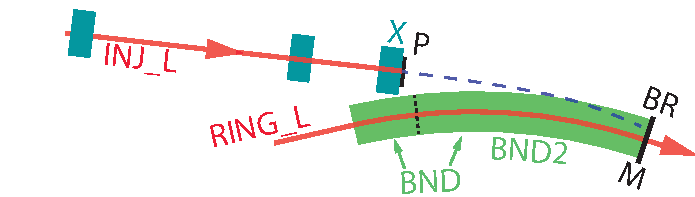
\includegraphics[width=5in]{injection.pdf}
  \caption[Injection line into a dipole magnet.]{
Injection line into a dipole magnet.
  }
  \label{f:inject}
\end{figure}

An injection line is illustrated in \fig{f:inject}. In this example,
The path of an injected particle after it leaves the last element
\vn{X} of the injection line (dashed blue line) partially goes through
the field of the dipole \vn{BND} in the storage ring. One way to
simulate this is:
\begin{example}
  INJ_L: line = (..., X, P, BND2, BR)
  RING_L: line = (..., BND, M, ...)
  P: patch, x_offset = -0.5, x_pitch = 0.15, z_offset = 0.3 
  BND: sbend, l = 6.2, g = 1/52
  BND2: BND, l = 4.7, tracking_method = runge_kutta,
          field_calc = fieldmap, grid_field = \{...\}
  BR: fork, to_line = RING_L, to_element = M
  M: marker
  use, INJ_L
\end{example}

In order to properly track particles through the fringe field of the
dipole \vn{BND}, a partial section of \vn{BND}, called \vn{BND2}, is
placed in the injection line \vn{INJ_L}. The \vn{tracking_method} for
\vn{BND2} is set to \vn{runge_kutta} since the default
\vn{bmad_standard} tracking is not able to handle these fringe
fields. Additionally, the \vn{field_calc} parameter of \vn{BND2} is
set to \vn{field map} so that the actual field profile of this particular
magnet can be used in the tracking. The field is specified in the
\vn{grid_field} parameter (\sref{s:fieldmap}). 

After traversing element \vn{X} in the injection line, the particle
goes through the patch \vn{P} which offsets the reference trajectory
so that following element, \vn{BND2}, is properly positioned.  The
beginning of \vn{BND2} is marked by a black dashed line in the figure.
At the end of \vn{BND2} the fork element \vn{BR} connects \vn{INJ_L}
with the marker \vn{M} in \vn{RING_L}.

%-----------------------------------------------------------------------------
\section{Example: Energy Recovery Linac}
\label{s:ex.erl}

An Energy Recovery Linac (ERL) is illustrated in \fig{f:erl}A. The ERL
starts with an injection line that feeds a linac which accelerates the
beam to some energy. The beam then transverses a return \vn{arc} which
reinjects the bunches into the linac. The length of the return arc is
such that, on the second pass, the beam is decelerated giving its
energy back to the RF cavities. Finally, the decelerated beam is
steered through a dump line where, at the end, an absorber stops the
beam.

 A lattice file for modeling this ERL:
\begin{example}
  parameter[geometry] = open
  parameter[absolute_time_tracking] = T

  BEND_L1: sbend, angle = -25*pi/180, l = 0.2, ...
  BEND_L2: BEND_L1

  A_PATCH: patch, flexible = T
  D_PATCH: patch, x_offset = 0.034, x_pitch = asin(0.32) 
  INJECT: line = (...)
  LINAC: line[multipass] = (BEND_L1, ..., BEND_L2)
  ARC: line = (..., BEND_A7)
  DUMP: line = (...)

  ERL: line = (INJECT, LINAC, ARC, A_PATCH, LINAC, D_PATCH, DUMP)
\end{example}

\begin{figure}[tb]
  \centering
  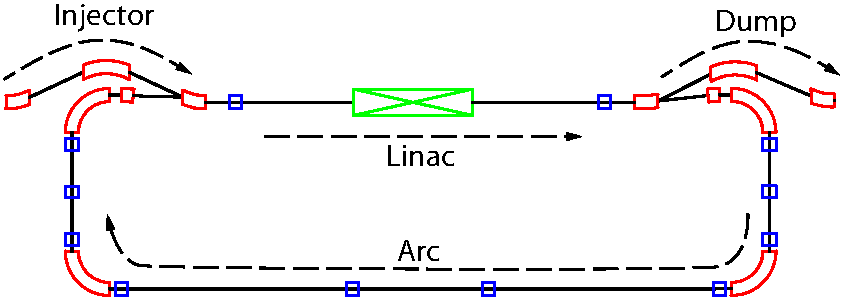
\includegraphics[width=6in]{erl.pdf}
  \caption[Example Energy Recovery Linac.]{
Example Energy Recovery Linac. A) The ERL consists of an injection line, accelerating linac, return
arc, deceleration linac, and finally a beam dump. B) Close up of the section where the end of the
injector and the end of the arc inject into the beginning of the linac. C) Close up of the end of
the linac which injects into the dump and the beginning of the arc.}
  \label{f:erl}
\end{figure}

\index{patch!example}
\fig{f:erl}B shows the injector and arc merging into the beginning of the linac. The first element
of the linac is a bend named \vn{BEND_L1}. The bending angle for \vn{BEND_L1} has been set at the
appropriate value for injection from the injector. To get the correct geometry for injection from
the arc, a \vn{patch} element, named \vn{A_PATCH}, is placed in the \vn{ERL} line between the arc
and the linac. \vn{A_PATCH} is a flexible patch which means that the exit edge of \vn{A_PATCH} will
automatically be aligned with the entrance edge of the next element which is \vn{BEND_L1}.

Note that this use of a flexible patch works since the orientation of \vn{BEND_L1} has been
determined before the orientation of \vn{A_PATCH} is determined. The orientation of elements is
determined in order starting from the first element in the line (the exception to this rule is if
there is a \vn{floor_position} element) and the orientation of \vn{BEND_L1} is thus determined right
after the injector section on the first pass through the linac.

\fig{f:erl}C shows the end of the linac splitting off into the dump and arc sections. The
\vn{D_PATCH} is used to orient the reference trajectory so that the dump is correctly positioned.
Here it is not possible to make the \vn{D_PATCH} flexible since the position of the dump is unknown
when the orientation of the \vn{D_PATCH} is calculated. However, the \vn{D_PATCH} could be made
flexible if a \vn{floor_position} element is used in the dump line (\bmad will work both forward and
backwards from a \vn{floor_position} element so that a \vn{floor_position} element may be placed
anywhere in the dump line).

%-----------------------------------------------------------------------------
\section{Example: Patch Between reversed and non-reversed elements}
\label{s:ex.patch}

\begin{figure}[tb]
  \centering
  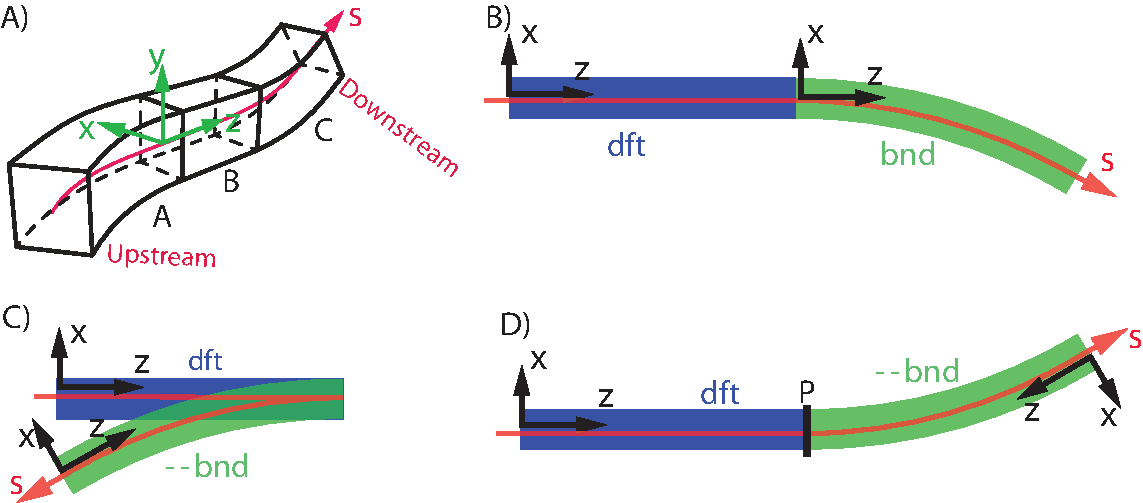
\includegraphics[width=5in]{patch-between.pdf}
  \caption[Patching between reversed and non-reversed elements.]{
Drift element \vn{D} is followed by a reversed drift element \vn{B}.  The view is from $+y$ onto the
$x$-$z$ plane. A) If no patch is present then the geometry does not make physical sense. B) With a
patch in between, a sane geometry can be obtained.}
  \label{f:patch.between}
\end{figure}

\index{patch}
Between normal and reversed elements there must be a reflection
\vn{patch} element (\sref{s:patch}).  This is illustrated in
\fig{f:patch.between}. The basic lattice is
\begin{example}
  D: drift, l = 2
  g_design = pi/12
  B: sbend, l = 2, g = g_design, g_err = -2*g_design
  P: patch, x_pitch = pi
  A_line: line = (D, --B)     ! Illegal. Do not use!
  B_line: line = (D, P, --B)  ! Correct
\end{example}
Line \vn{A_line} represents the situation shown in \fig{f:patch.between}A.  With no patch between
the drift \vn{D} and the reversed bend \vn{B}, a particle leaving \vn{D} at \vn{D}'s downstream end
will find itself outside of both \vn{D} and \vn{B}. Clearly this is an unphysical situation. Sanity
is restored in line \vn{B_line} shown in \fig{f:patch.between}B. In this instance, the patch \vn{P}
rotates the reference coordinates around the $y$-axis leaving the $y$-axis invariant the bend of
\vn{B} is in the $x$-$z$ plane. There are other patch parameter values that could be used to produce
a reflection patch (\sref{s:reflect.patch}).  For example, Setting the patch's \vn{y_pitch} to
\vn{pi} would produce a reflection patch.

Since bend \vn{B} is reversed, A particle moving downstream within \vn{B} is going the opposite
direction from the normal direction. If \vn{g_err} were zero in this instance, a downstream moving
particle would feel a force that will rotate the particle in a clockwise manner opposite from the
counterclockwise direction of the bend. To counter this, \vn{g_err} is set so the total bending
field \vn{g_tot = g + g_err} is opposite the design field. That is, \vn{g_err} is set so that
\vn{g_tot = -g}.

%-----------------------------------------------------------------------------
\section{Example: Colliding Beam Storage Rings}
\label{s:ex.collide}

\begin{figure}[tb]
  \centering
  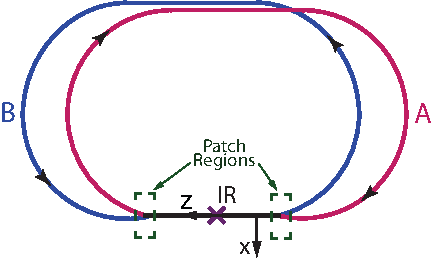
\includegraphics[width=5in]{colliding-beams.pdf}
  \caption[Dual ring colliding beam machine]{Dual ring colliding beam machine. 
The beam in the \vn{A} ring rotates clockwise and in the \vn{B} ring
counterclockwise.}
  \label{f:collide}
\end{figure}

The idealized layout of a pair of storage rings used for colliding
counter rotating beams of electrons and gold is shown in \fig{f:collide}. Rings \vn{A} and
\vn{B} intersect at two interaction regions labeled \vn{ir1} and
\vn{ir2} where the beams collide. The basic lattice description is:
\begin{example}
  ir: line[multipass] = (...)
  pa_in; patch, ... ;  pa_out; patch, ...
  pb_in; patch, ... ;  pb_out; patch, ...
  m: marker
  fid: fiducial, origin_ele = m
  ...
  A: line = (arc_a, pa_in, ir, m, pa_out)
  A[particle] = electron
  B_rev: line = (arc_b, pb_in, ir, fid, pb_out)
  B: line = (--B_rev)
  B[particle] = Au+79
  use, A, B
\end{example}
Lines \vn{ir} is the interaction region line which is
declared \vn{multipass} since they are shared by the two rings. Line
\vn{A} represents ring \vn{A}. In ring \vn{A} where the electron beam which, by definition,
travels in the same direction as increasing $s$, rotates clockwise.
Line \vn{B_rev} is a ``reversed'' line of ring \vn{B} and, like
\vn{a}, represents a beam rotating clockwise.  Line \vn{B}, which
represents ring \vn{B}, is the reverse of \vn{B_rev} and here the gold beam
rotates counterclockwise. In this construction, all elements of \vn{B}
are reversed.  While this is not mandatory (only the interaction
regions must be reversed in \vn{B}), having all of \vn{B} reversed
simplifies the geometry since this means that the local coordinate
systems of both lines \vn{A} and \vn{b} will be ``aligned'' with the
$x$-axis pointing to the outside of the ring and the $y$-axis pointing
up, out of the page. Having non-aligned coordinate systems is possible
but potentially very confusing.

The two rings are physically aligned using a marker \vn{m} in \vn{A}
and a \vn{fiducial} element \vn{fid} in \vn{B} that aligns with
\vn{m}.  Each ring has two rigid \vn{patch} elements, \vn{pa_in} and \vn{pa_out} for the \vn{A}
ring, and \vn{pb_in} and \vn{bp_out} for the \vn{B} ring, on either side of the interaction region.
The dashed, green rectangles in the figure show the regions where the patches are.

The finished lattice will have two branches, The first branch (with
index 0) will be derived from line \vn{A} (and hence will be named
``A'') and the second branch (with index 1) will be derived from line
\vn{B} (and hence will be named ``B''). The multipass lords
representing the physical IR elements will be in the ``lord section''
of branch 0.



\begin{figure}[tb]
  \centering
  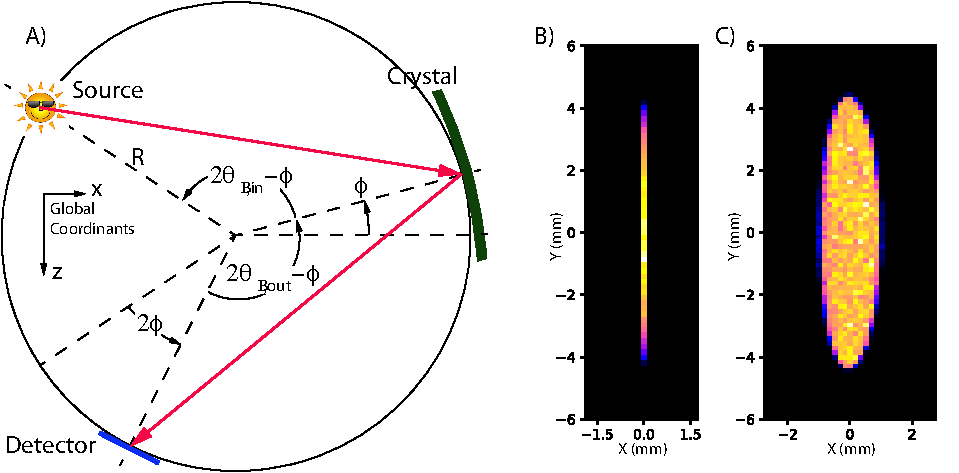
\includegraphics[width=5in]{rowland-circle.pdf}
  \caption[Rowland circle spectrometer]
  {
Rowland circle spectrometer: A) X-rays scattered from a sample (labeled source in the figure)
illuminates a crystal with X-rays. Some of the X-rays are reflected from the crystal onto the
detector. Note: For clarity's sake the center of the global coordinate system as shown is shifted
from the true center at the Source element. B) The detector image when the radius of curvature of
the bent crystal is ``perfect''. That is, twice the radius of the Rowland circle. C) The detector
image when the radius of curvature of the crystal is shifted 1\% from perfect.
  }
  \label{f:rowland}
\end{figure}

%-----------------------------------------------------------------------------
\section{Example: Rowland Circle X-Ray Spectrometer}
\label{s:rowland}

This example shows how \bmad can be used to simulate X-rays. In this case, the present example is
taken from a case study where simulations were done in order to understand how imperfections in a Rowland
circle spectrometer would affect measurements.

A Rowland circle spectrometer is illustrated in \fig{f:rowland}A. The \vn{source} was
a sample that is illuminated with X-rays. Some of the X-rays scatter from the \vn{sample} and are
reflected from the \vn{crystal} to the \vn{detector}. To properly focus the X-rays onto the
\vn{detector}, the \vn{source}, \vn{crystal} and \vn{detector} lie on a circle, called the Rowland
circle. The \vn{crystal} is bent and the radius of curvature of the crystal is
$2R$ where $R$ is the radius of the Rowland circle.

The angle from the \vn{source} to the Rowland circle center to the crystal is
$2\theta_\text{B,in}-\phi$ where $\theta_\text{B,in}$ is the entrance Bragg angle for photons whose
energy matches the given reference energy and $\phi$ is an angle that will be varied when doing an energy
scan of the scattered X-ray spectrum. Similarly, the angle from the \vn{crystal} to the Rowland
circle center to the \vn{detector} is $2\theta_\text{B,out}-\phi$ where $\theta_\text{B,out}$ is the
exit Bragg angle at the given reference energy.

The lattice for this simulation is:
\begin{example}
  beginning[e_tot] = 8.955e3    ! Reference photon energy
  parameter[particle] = photon

  phi = 0
  err = 0
  r_rowland = 0.5               ! Rowland circle radius

  source: photon_init, sig_x = 5e-5, sig_y = 5e-5, spatial_distribution = uniform,
          E_center_relative_to_ref = T, sig_E = 2, energy_distribution = gaussian,
          velocity_distribution = spherical

  drift1: drift

  cryst: crystal, crystal_type = 'Si(553)', b_param = -1, aperture = 0.050,
  	spherical_curvature = (1+err) / (2 * r_rowland), aperture_type = elliptical

  drift2: drift

  det: detector, surface = \{grid = \{ix_bounds = (-97, 97), 
                                    iy_bounds = (-243, 243), dr = (172e-6, 172e-6)\}\}

  daves_line: line = (source, drift1, cryst, drift2, det)
  use, daves_line

  !------------------

  expand_lattice ! Calculates the Bragg angles needed below.

  theta_in  = cryst[bragg_angle_in]  ! 78.2759 * pi / 180
  theta_out = cryst[bragg_angle_out] ! 78.2759 * pi / 180

  cryst[graze_angle_in]  = theta_in - phi/2 
  cryst[graze_angle_out] = theta_out - phi/2
  drift1[L] = 2 * r_rowland * sin(theta_in-phi/2)
  drift2[L] = 2 * r_rowland * sin(theta_out-phi/2)

  beginning[theta_position] = theta_in + phi/2
  det[x_pitch] = pi/2 - theta_out + phi/2
\end{example}

The reference photon energy is 8.995~KeV and the Rowland circle radius is 0.5~m. The simulation uses
a \vn{photon_init} element (\sref{s:photon.init}) for the \vn{source} having a Gaussian energy
spread with a sigma of 2~eV.  The initial velocity distribution of the photons, set by the
\vn{velocity_distribution} parameter, is taken to be uniform in all directions (``\vn{spherical}''
distribution). Since the element that is downstream from the source (which is the crystal element)
has a defined aperture, \bmad is able to use this to not generate photons that will be lost at the
crystal. This reduces the simulation time.

The crystal is \vn{Silicon} 553 crystal which is symmetrically cut (\vn{b_param} = -1) so that in
this example the entrance Bragg angle is equal to the exit Bragg angle.  The detector has a
segmented surface with pixels spaced 172$\mu$m apart. Along the $x$-axis, which is the coordinate
along the detector surface in the plane of \fig{f:rowland}A, the pixel index is in the range $[-97,
97]$. Along the $y$-axis, which is the out of plane coordinate, the pixel index is in the range
$[-243,243]$.

The \vn{expand_lattice} command (\sref{s:expand.lat}) is used to command \bmad to construct the
lattice which includes calculating the Bragg angles. After lattice expansion, the variables
\vn{theta_in} and \vn{theta_out} are set to the Bragg angle entrance and exit Bragg angles
respectively. The entrance and exit graze angles of the crystal, which are used to determine the
reference trajectory (\sref{s:mirror.coords}, can be set to \vn{theta_in - phi} and \vn{theta_out -
phi} respectively. Note that if these graze angles had not been explicitly set, the graze angles
would be automatically set to the Bragg angles which
is not what is wanted when doing an energy scan with finite \vn{phi}.

In the actual experimental setup that this example is modeled on, the source and Rowland circle were
fixed in the global coordinate system (\sref{s:global}) while the crystal and detector move with
changing \vn{phi} (see \fig{f:rowland}A). To mimic this, the \vn{beginning[theta_position]}
(\sref{s:beginning}) is set to give the desired orientation of the beginning reference trajectory
within the global coordinate system. This does not affect photon tracking since changing the initial
orientation of the reference trajectory just shifts all the lattice elements as one rigid
body. Additionally, the detector orientation is fixed so that the detector surface normal always
points towards the Rowland circle center. To get the correct orientation for the detector, the
detector's \vn{x_pitch} attribute, which rotates the detector (\sref{s:offset}), is set appropriately.

The effect of varying the \vn{crystal} curvature is shown in \fig{f:rowland}B and
\fig{f:rowland}C. A \bmad based program called \vn{Lux} was used for the simulation. The \vn{Lux}
program generates a set of photons and records the statistics at the detector. In \fig{f:rowland}B
the \vn{crystal} is correctly bent with the parameter \vn{err} in the lattice set to zero. This
produces a well focused spot on the \vn{detector}. In \fig{f:rowland}C the \vn{crystal} curvature
is shifted by 1\% by setting \vn{err} equal to 0.01. This error degrades the focusing and leads to a
spot that is enlarged along the $x$-axis.


%-----------------------------------------------------------------------------
\section{Example: Backward Tracking Through a Lattice}
\label{s:reverse}

By creating a reversed lattice, one can essentially track particles backwards. For example,
assume that you have a lattice file called \vn{original_lattice.bmad} which defines a line
called \vn{original_line}. To create a reversed lattice, create a new file with the following:
\begin{example}
  call, file = original_lattice.bmad
  reversed_line: line = (--original_line)
  parameter[particle] = antiparticle(parameter[particle])
  use, reversed_line
\end{example}
The ``\vn{--}'' reverses the line and reverses the elements (\sref{s:ele.reverse}). Tracking through
\vn{reversed_line} is equivalent to tracking backwards through \vn{original_line}.  

If the \vn{original_line} lattice had just static magnetic fields and no electric fields, then
by tracking with the anti-particle in the reversed lattice, the anti-particle will follow the same
path (but backward) as the the particle in the original lattice. For this to work, the anti-particle
must be started with the appropriate phase space coordinates. If $(x, p_x, y, p_y, z, p_z)$ is
the phase space coordinates of the particle at the end of the original lattice, the anti-particle
must be initialized with phase space coordinates of $(x, -p_x, y, -p_y, \text{immaterial}, p_z)$.
